\subsubsection{React}

Основной концепцией React является разбиение элементов приложения на компоненты. Компонентами в данном случае являются небольшие фрагменты страниц. На рисунке~\ref{img:react__components} приведён пример разбиения страницы на компоненты. Для примера была выбрана страница поиска Google.

\begin{figure}[H]
  \centering
  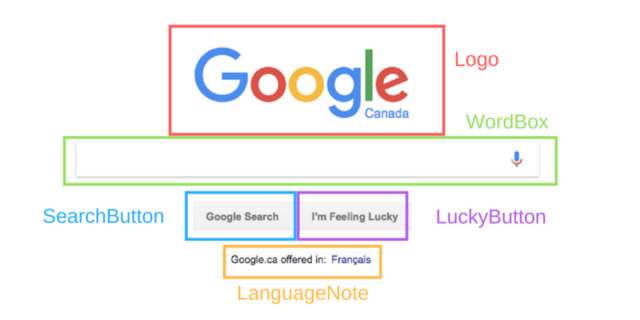
\includegraphics[width=0.9\textwidth]{assets/images/theoretical2/components.png}
  \caption{Разбиение страницы на компоненты}
  \label{img:react__components}
\end{figure}

Компонент React представляет из себя участок кода, соответствующий части веб-страницы приложения.

По умолчанию, точкой входа React приложения является контейнер div с идентификатором Root. В этом контейнере будет содержаться всё веб приложение. Веб приложение при этом будет представлять из себя композицию компонентов или JSX элементов, состоящих из одного или нескольких компонентов или JSX-элементов.

Данные в компоненте хранятся в виде <<пропсов>>. Они представляют собой один объект, в котором перечислены все используемые данные~\cite{react}. Также пропсы можно передавать дочерним компонентам, указывая какие данные передаются. Например, на рисунке~\ref{img:react__props} представлен JSX элемент, состоящий из компонента Welcome, в который передаётся пропс name со значением <<Алиса>>.

\begin{figure}[H]
  \centering
  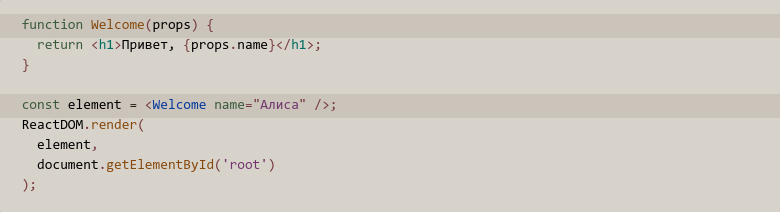
\includegraphics[width=0.9\textwidth]{assets/images/theoretical2/props.png}
  \caption{Передача пропсов}
  \label{img:react__props}
\end{figure}

На рисунке~\ref{img:react__components_composition} представлен пример React приложения, состоящий из компонентов Welcome с разными входными параметрами, вложенных в компонент App, подключаемый к контейнеру с идентификатором root. Компонент Welcome при этом представляет собой JSX элемент, соответствующий заголовку h1 HTML.

\begin{figure}[H]
  \centering
  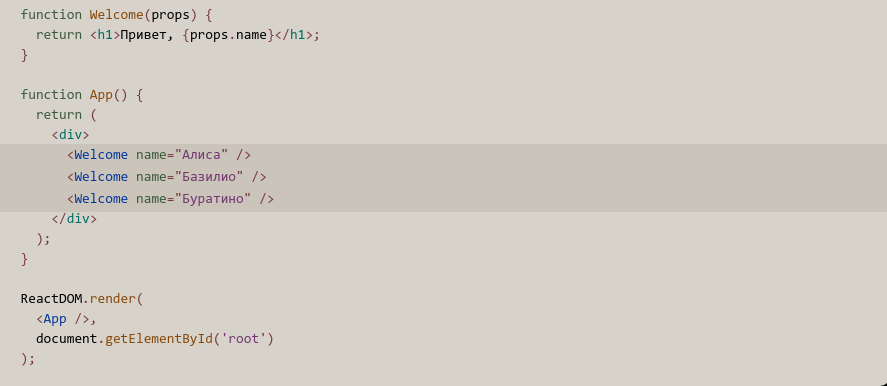
\includegraphics[width=0.9\textwidth]{assets/images/theoretical2/components__composition.png}
  \caption{Композиция React компонентов}
  \label{img:react__components_composition}
\end{figure}

Результатом отображения кода на рисунке~\ref{img:react__components_composition} будет веб страница, предложенная на рисунке~\ref{img:react__components_composition-result}.

\begin{figure}[H]
  \centering
  
\includegraphics[height=0.25\textheight]{assets/images/theoretical2/components__composition-result.png}
  \caption{Результат отображения композиции React компонентов}
  \label{img:react__components_composition-result}
\end{figure}